\documentclass[11pt,a4paper]{report}

\usepackage[margin=3cm]{geometry}
\usepackage{graphicx}
\usepackage{amsmath,amsfonts,amssymb}
\usepackage{url}
\usepackage{booktabs}
\usepackage{array}
\usepackage{multirow}
\usepackage{caption}
\usepackage{float}
\usepackage[hidelinks]{hyperref}
\usepackage[backend=biber,style=numeric]{biblatex}

\addbibresource{references.bib}

\title{An Empirical Analysis of JavaScript Framework Overhead for NLP-Based Educational Web Applications Under Simulated Classroom Computing Constraints}
\author{Kavitharshan Baskaran}
\date{September 2026}

\begin{document}

% ============================================================
\begin{titlepage}
\centering
\vspace*{2cm}



\includegraphics[width=4cm]{figures/warwick-crest.jpeg}


\vspace{1.5cm}

{\Large \textbf{An Empirical Analysis of JavaScript Framework Overhead for NLP-Based Educational Web Applications Under Simulated Classroom Computing Constraints}}

\vspace{2cm}

by

\vspace{0.5cm}

{\large Kavitharshan Baskaran}

\vspace{3cm}

Department of Computer Science\\
University of Warwick

\vspace{1cm}

September 2026

\vfill

CS907/CS913 Dissertation Project\\
Supervisor: Dr. Mike Joy

\end{titlepage}

% ============================================================
\begin{abstract}

This dissertation investigates whether the choice of frontend JavaScript framework measurably affects the performance of a realistic, NLP driven educational web application under simulated classroom computing constraints. Three functionally and visually identical implementations were created, using Vanilla JavaScript, React, and Angular respectively. These implementations were built around an identical backend serving a pretrained CEFR text classifier, and benchmarked using an automated Playwright harness across three simulated hardware/network environments, four usage scenarios,
and four performance metrics, totaling 1,080 individual runs. Results were analysed using Kruskal-Wallis tests with Bonferroni correction, pairwise Mann-Whitney U tests and Cohen's d.

\vspace{5mm}

Frontend framework choice was found to produce a statistically significant difference in application responsiveness across every scenario, environment, and metric tested. Vanilla JavaScript performed best overall, Angular consistently outperformed React on Time-to-Result while recording the highest peak heap memory of the three. A significant finding of this study is that Environmental constraint had a substationally larger effect on performance than framework choice itself, though one exception was found under repeated interaction. A further finding showcased that Time-to-Interactive degrades under throttling almost independently of framework, whereas Time-to-Result does not, indicating the latter is the more informative metric for studies of this kind. These findings extend, and in places contradict, existing framework comparisons conducted on unconstrained, developer-grade hardware, highlighting the value of evaluating frontend performance under conditions that reflect real classroom deployment. 


\end{abstract}

\tableofcontents
\listoffigures
\listoftables

% ============================================================
\chapter{Introduction}
\label{ch:introduction}

What happens when a user isn't on a £2000 laptop? This question lies at the heart of modern web development, where the gap between developer hardware and user reality is becoming more and more distinguishable. A developer in London builds an application on a 32GB MacBook, while the intended users open it on a 4GB tablet. What seems snappy on one end may not be mirrored to the other side. 

\section{Motivation}

Rapid advancements in digital technologies have ushered the modern web a long way from the static, document-based pages of its earlier years. The time a webpage could have simply been a fixed piece of text and markup has been replaced by an expectation of dynamic, interactive, application-like experiences that rival native software. This shift has fundamentally altered how developers build for the web, and how users expect it to behave. Today's web applications are built as sophisticated, interactive programs which run a substantial amount of JavaScript directly in the user's browser, including operations such as
fetching data, updating the interface in real time, and managing complex application states entirely on the client side. 

\vspace{5mm}

This architectural evolution has yielded undeniable benefits across the digital ecosystem, users are now able to interact with applications that feel responsive and capable, usually without ever leaving their browser. However, this leap in capability has introduced new challenges. The very abstractions that enable the rapid development and rich user experiences which underpin modern frontend engineering also introduce overhead. This transition from document-centric to application-centric web development proliferated the widespread adoption of frontend frameworks, as the increasing complexity of modern web applications demanded
structured approaches to managing application state, user interfaces, and interactions~\cite{johnson1997}. React and Angular have emerged as prominent examples of distinct architectural philosophies, with React advocating a unidirectional data flow and virtual DOM, whilst the latter favours more of an opinionated, dependency-injected architecture. Every layer of abstraction adds instructions, every component lifecycle adds computation, and every dependency adds weight, this shift has made it practical to embed increasingly sophisticated functionality directly into web tools without hand-writing every DOM update. 

\vspace{5mm}

Education has been one of the clearest recipients of this great technological shift, with students and teachers alike depending web-based tools including automated writing feedback tools, intelligent tutoring systems, and adaptive learning platforms. These applications are no longer limited to users with access to proprietary software, and are now widely accessible and deployable as ordinary web applications. This opens up access for a wider audience, to capabilities that were previously expensive or impractical. However, a design decision that is
often taken for granted when building such tools is the choice of frontend framework itself. Framework selection is frequently driven by developer familiarity, ecosystem popularity, or team convention, rather than by empirical evidence of how that choice affects the experience of the tool's actual end users.

\vspace{5mm}

This gap matters significantly in an educational context. Existing frontend benchmarks, most notably the widely cited js-framework-benchmark project, typically measures narrow, simple operations such as creating list items or re-ordering table rows, usually whilst on developer grade hardware with fast, stable networks. This poorly represents the conditions faced in many real classrooms, where shared, ageing Chromebooks, and congested school Wi-Fi, are the norm rather than the exception.  A
framework that performs indistinguishably from its alternatives on a developer's own machine may behave very differently once realistic CPU throttling and network latency are introduced. Framework choices made without this knowledge risks quietly disadvantaging exactly the students who can least afford a sluggish, unresponsive tool. There is, therefore, a clear need for proper empirical evaluation of frontend performance under conditions that correctly represent classroom deployment, rather than 
developer conditions.


\section{Research Question}

This dissertation delves into the question of whether the choice of frontend framework measurably affects the performance of a realistic, NLP-driven educational web application when run under simulated classroom constraints. The frameworks under comparison are React and Angular, two of the most widely adopted frontend frameworks in the industry, with Vanilla JavaScript employed as a baseline in order to isolate framework specific overhead from the intrinsic computational demands inherent to the underlying task itself. 

\vspace{5mm}

Rather than constructing a generic benchmark, each implementation performs a genuinely useful task, the automatic classification of student writing by CEFR (Common European Framework of Reference for Languages) proficiency level using a pretrained transformer-based classifier. This ensures that the performance evaluation reflects a meaningful, educationally relevant workload, whilst also providing a realistic asynchronous pipeline that encompasses text submission, network request, model inference, and UI update. This way, the benchmark faithfully represents the kind of application architecture that is increasingly deployed in real world educational settings. 

\vspace{5mm}

Building on this motivation, the project addresses three specific research questions. Formally, these research questions are framed as:

\begin{enumerate}
  \item How do Vanilla JavaScript, React, and Angular differ in load-time
  performance when delivering an NLP-based educational tool, and does the
  magnitude of this difference change across varying device
  specifications?
  \item How do Vanilla JavaScript, React, and Angular differ in runtime
  memory consumption and Time-to-Result during NLP inference interactions,
  and at what level of hardware constraint do these differences become
  significant?
  \item Is there a device specification or constraint threshold below
  which any framework with non-trivial runtime overhead becomes unsuitable
  for delivering responsive feedback in a classroom setting?
\end{enumerate}

Three functionally identical implementations of the same application were built, one in each framework, sharing an identical backend and visual design, so that any measured performance difference observed can be attributed specifically to the frontend framework rather than to confounding factors such as differences in layout, styling, or backend behaviour.

\section{Contributions}

This dissertation proposes to make the following four contributions:

\begin{enumerate}
  \item Three functionally identical implementations of an NLP-driven
  educational web application (Vanilla JavaScript, React, Angular),
  sharing an identical backend and visual design, publicly available on
  GitHub.
  \item A reusable, automated benchmarking harness built with Playwright
  and the Chrome DevTools Protocol, capable of simulating three
  classroom-representative hardware/network environments and capturing
  four performance metrics across four distinct usage scenarios.
  \item A dataset of 1,080 individual benchmark runs, analysed using
  non-parametric statistical methods (Kruskal-Wallis, pairwise
  Mann-Whitney U with Bonferroni correction, Cohen's d) to determine
  whether, and to what extent, frontend framework choice affects
  application performance under constrained conditions.
  \item An empirical answer to the research question above, along with a
  characterisation of how the performance gap between frameworks changes
  as hardware and network constraints intensify (the degradation
  gradient).
\end{enumerate}


% ============================================================
\chapter{Background and Research}
\label{ch:background}

This chapter presents a literature review that establishes the theoretical and technical context for the empirical work that follows, covering existing research relevant to the two distinct areas this project draws on, frontend framework performance and automatic CEFR classification. For each study, the methodology employed is described, key findings are reported, and limitations are identified that motivate specific design decisions taken in this project. Portions of this chapter develop and expand upon the literature review first presented in the Interim Report.  

\section{Frontend Framework Performance Benchmarking}
\subsection{js-framework-benchmark}

The field of frontend framework performance has been extensively researched, though existing approaches typically rely on operation-level benchmarks rather than realistic, application and hardware level workloads. The most widely referenced example of this is Krause's \texttt{js\allowbreak-framework\allowbreak-benchmark} ~\cite{krause}, an open-source project that measures the duration of isolated DOM operations, specifically creating,
updating, selecting, and removing rows in a large table across a very large number of framework implementations (over 180), using a Selenium-driven webdriver harness to gather timing data directly from the browser. This methodology produces a valuable, low-level comparator of DOM reconciliation speed, its scale and continued maintainance give it significant credibility in the field. However, it deliberately isolates rendering performance from real application concerns, explicitly excluding backend response handling and asynchronous network request handling, and is run exclusively on developer-grade hardware. This reveals a gap this dissertation is positioned to address directly, js-framework-benchmark 
provides important insight into DOM reconcillation speed specifically, but does not address how frameworks behave under a realistic request/response lifecycle, or under constrained hardware/network conditions. 

\subsection{Chhetri's Comparative Study of React and Angular}

Chhetri~\cite{chhetri} conducts a direct comparative study of React and Angular, employing a methodology closely related to the one used in this project. Chhetri built identical applications in both frameworks, tested using Lighthouse for performance profiling, Chrome DevTools for standardised web-performance metrics, and browser-based memory analysis tools. Chhetri reported that React achieved a 63\% faster First Contentful Paint than Angular, and a 40\% reduction in peak heap size. This finding is backed up by Emmanni~\cite{emmanni}, whose independent comparison of Angular, React, and Vue.js reported a similar ordering for load time, though Emmanni also notes that Angular's strength in large-scale project tooling and TypeScript integration as a separate, non-performance consideration. Together, these two studies are directly relevant to this project's own results (Chapter~\ref{ch:results}), which found the opposite ordering for Time-to-Result, Angular consistently outperformed React across nearly every condition tested. However React suprisingly recorded the second highest peak heap memory. This contrast is unique to this dissertation project and is worth confronting. Both Chhetri and Emmanni evaluated a single simple application, tested once on developer-grade hardware, with no
repeated measurement and no statistical testing to establish whether observed differences reflect a genuine effect or measurement noise. Neither of the studies implementation includes any asynchronous network workload comparable to this dissertation project's backend classification request. This dissertation projects use of asynchronous NLP workload, 30 repetitions per condition, and non-parametric significance testing represents a direct methodological improvement over both authors approaches.

\subsection{Comparative Performance-Efficiency Studies}

Expanding the comparative framework analysis even further, Loja and Maita~\cite{loja-maita} evaluate Angular, React, and Vue.js against the ISO/IEC 25010 software quality model, focusing specifically on the temporal behaviour and resource utilisation sub-characteristics of performance efficiency. This study's use of an established international standard to structure its evaluation gives it a degree of methodological rigour that many informal framework comparisons lack. However, similar to Chhetri's study, evaluation was conducted on a single application under a single, unconstrained hardware condition, and the study does not report statistical significance testing across repeated trials. A broader comparative study by \cite{comparative-frameworks} also evaluates React, Angular, and Vue.js against different load conditions and scalability scenarios, finding that Angular's richer feature set increases load time and memory usage relative to the other two frameworks, which this dissertation project's results have also reproduced for peak heap memory, lending some corroborating weight to that specific finding. Much like the previous studies, this comparison was conducted exclusively on developer-grade hardware, and does not examine how these performance differences may change, or amplify, under resource-constrained conditions. 

\vspace{5mm}

Across each of the five framework-comparison studies reviewed in this section, none of them report statistical significance testing or effect-size analysis across repeated measurements. Each reports single-run or small-sample findings directly, without explicit treatment of measurement variance. This dissertation project addresses this gap through the employment of the 30 repetitions per condition strategy and non-parametric hypothesis testing, which is described in Chapter~\ref{ch:approach}. 

\section{Web Performance Under Constrained Hardware and Networks}
\subsection{MAML and Low-End Device Performance}

The question of web performance under constrained hardware and network conditions has been studied directly, though typically outside the context of framework comparison specifically. Pandey et al.~\cite{maml} document that growing webpage complexity and JavaScript reliance in particular disproportionately affects users on low-end devices with limited bandwidth, leading to longer load times and more frequent unresponsiveness. Their proposed solution, MAML, is an alternative, lightweight web specification language designed to reduce the JavaScript and CSS payload delivered to constrained devices. While MAML addresses this problem by replacing conventional web technologies altogether, it neither asks or answers a narrower, more practically oriented question that motivates this dissertation project, Given a development team is already committed to using a conventional JavaScript framework, does the specific choice of framework meaningfully affect the experience of users on constrained devices and by how much? Pandey et al.'s finding  
that JavaScript payload size is a primary driver of degraded performance on low-end devices directly motivates the inclusion of bundle size as one of this project's four measured metrics. 

\vspace{5mm}

None of the framework-comparison studies reviewed in Chapter~\ref{ch:background} test under conditions resembling those described by Pandey et al., leaving open the specific question this dissertation project investigates, whether the framework-level differences reported by Chhetri, Loja and Maita, and others persist, widen, or narrow once realistic hardware and network constraints of the kind MAML describes are introduced.

\section{Automatic CEFR Classification}

\subsection{Transformer-Based Approaches}

The NLP component of this project employs automatic CEFR-level classification to provide the basis for a realistic and educationally meaningful workload, this is itself a well-established research task. Lagutina et
al.~\cite{cefr-ml} conducted a comprehensive evaluation of both classical machine learning classifiers and BERT-based models for this purpose, finding that BERT-based models achieve strong performance, with an F-score of 69\% when
classifying text across proficiency levels.

\subsection{Classical vs. Machine Learning Methods}

Lagutina et al.'s work also provided useful qualitative insight. Classification errors were observed to be more frequent between adjacent CEFR levels, for example with B1 misclassified as B2, this pattern is consistent with the inherent subjectivity of neighbouring proficiency bands. Their findings confirm both the effectiveness of automatic CEFR classification and its practical vialbility for e-learning systems, reinforcing its suitability as a realistic workload for this project. These findings directly inform the choice of a fine-tuned transformer-based classifier (\texttt{theluantran/cefr-bert-classifier}) as the NLP component.


\section{Identified Research Gap}

The literature reviewed above reveals a clear gap that this dissertation project has manoevoured itself into a position to address. While Direct framework performance comparisons do exist~\cite{krause,chhetri,emmanni,loja-maita,comparative-frameworks}, each was conducted on developer-grade hardware with a single application and no statistical treatment of measurement variance, and none tests a genuinely asynchronous, network-dependent workload. Separately, web performance on low-end devices has been studied~\cite{maml}, but not specifically in the context of framework comparison. Neither body of work addresses the intersection this project investigates, how frontend framework choice 
affects the performance of a realistic NLP application under simulated classroom-representative hardware and network constraints., evaluated with repeated measurement and non-parametric statistical testing. This dissertation's contribution is to fill this gap through the use of a genuinely useful NLP workload~\cite{cefr-ml}, and a systematic, statistically validated comparison across multiple simulated hardware/network conditions, directly addressing the methodological limitations identified across the framework-focused studies reviewed in this chapter.


% ============================================================
\chapter{Approach}
\label{ch:approach}

This chapter describes the methodological approach taken to answer the research questions established in Chapter 1. It covers the requirements analysis, experimental design, technological decisions, and project planning underpinning the benchmarking study.

\section{Requirements Analysis}

The project's requirements were derived directly from the three research questions established in Chapter~\ref{ch:introduction}. Answering these questions rigorously imposed several concrete requirements on the system to be built: 

\begin{enumerate}
  \item \textbf{Functional equivalence across implementations.} For any measured performance difference to be attributable to framework choice alone, the three frontend implementations needed to be functionally and visually identical — sharing the same user interface, interaction flow, backend, and styling — and differing only in the framework used to implement them.
  \item \textbf{A realistic, non-trivial workload.} The application needed to perform a genuinely useful task involving asynchronous network communication, rather than a synthetic operation such as list rendering, so that the benchmark results generalise to real-world educational tools rather than to an artificial edge case.
  \item \textbf{Controllable, repeatable environment simulation.} To answer RQ1 and RQ2, which both ask how performance differences change across device specifications, the system needed a way to reliably reproduce multiple distinct hardware and network conditions, rather than relying on physically acquiring a range of real devices.
  \item \textbf{Statistically robust measurement.} A single measurement per condition would be vulnerable to noise from background system activity, garbage collection timing, and other transient effects. Multiple repetitions per condition, combined with appropriate statistical testing, were required to distinguish genuine framework effects from measurement noise.
  \item \textbf{Multiple performance dimensions.} RQ1 and RQ2 ask about load-time, memory consumption, and Time-to-Result specifically, requiring the system to capture more than one metric per run.
\end{enumerate}


\section{Experimental Design}

\subsection{Frameworks Under Test}

Three frontend implementations were built, with Vanilla JavaScript serving as a baseline with no framework overhead, React was chosen for its widespread industry usage and unidirectional, virtual-DOM-based architecture, and Angular was chosen for its constrasting dependency-injected architecture. This framework selection considers two of the most commonly used frontend frameworks alongside a zero-overhead baseline, allowing measured overhead to be compared against a true floor, rather than only against each other. 

\subsection{Simulated Environments (E1, E2, E3)}

In order to correctly represent a realistic spread of classroom hardware three environments were defined, moving from an unconstrained baseline similar to what a developer's workspace would be, to conditions that are typical of low-end, shared classroom devices:

\begin{enumerate}
  \item \textbf{E1 (Baseline):} No CPU or network throttling applied, representing developer-grade hardware and a fast, stable connection.
  \item \textbf{E2 (Mid-range mobile):} 4$\times$ CPU throttling, 5Mbps bandwidth, 100ms round-trip latency, representing a mid-range, several-year-old device on a moderately congested network.
  \item \textbf{E3 (Low-end mobile):} 6$\times$ CPU throttling, 5Mbps bandwidth, 100ms round-trip latency, representing an entry-level Chromebook processor on the same congested network.
\end{enumerate}   

These particular throttling values are not arbitrary and were considered to approximate the difference in single-core CPU performance between typical developer laptops and low-cost Chromebook processors commonly deployed in schools, combined with bandwidth figures representative of congested,
shared school Wi-Fi rather than a dedicated broadband connection.

\subsection{Test Scenarios}

Four distinct usage scenarios were defined, each exercising a different aspect of application performance:

\begin{enumerate}
  \item \textbf{Cold Load:} Measures pure page load and initialisation
  cost with no user interaction, isolating framework startup overhead
  from the cost of the NLP classification task itself.
  \item \textbf{Single Submission:} The primary, representative scenario:
  a single piece of text is submitted and classified, measuring the full
  end-to-end interaction a real user would experience.
  \item \textbf{Stress Test:} Five submissions are made in rapid
  succession, testing how each framework's state management behaves
  under repeated, closely-spaced interaction.
  \item \textbf{Error Handling:} The backend request is deliberately
  made to fail, measuring how quickly and reliably each frontend
  surfaces an error state to the user.
\end{enumerate}

\subsection{Performance Metrics}

Four metrics were captured for each individual run, directly addressing the performance dimensions covered in RQ1 and RQ2:

\begin{enumerate}
  \item \textbf{Time-to-Result (TTR):} End-to-end latency from form
  submission to a rendered result, the metric most directly experienced
  by an end user.
  \item \textbf{Time-to-Interactive (TTI):} A proxy measuring how quickly
  the page becomes ready for interaction after navigation, addressing the
  load-time dimension of RQ1.
  \item \textbf{Peak Heap Memory:} The maximum JavaScript heap usage
  observed during a run, addressing the runtime memory consumption
  dimension of RQ2 and relevant to the low-RAM devices RQ3 is concerned
  with.
  \item \textbf{Bundle Size:} The total compressed JavaScript payload
  delivered to the browser, relevant to network-constrained conditions
  such as E2 and E3.
\end{enumerate}

Each of the four scenarios were executed 30 times per framework/environment combination, giving $3 \text{ frameworks} \times 3 \text{ environments} \times 4 \text{ scenarios} \times 30 \text{ repetitions} = 1{,}080$ individual runs in total.

\section{Technological Decisions}

\subsection{Backend: FastAPI and the CEFR Classifier}

A local FastAPI backend was chosen to serve the CEFR classification model, wrapping \texttt{theluantran/cefr-bert-classifier}, a fine-tuned XLM-RoBERTa model. FastAPI was selected for its lightweight footprint, asynchronous request handling, and seamless integration with Python-based machine learning libraries, thus making it well-suited for the dissertation's need for a performant, locally-runnable API. By running the model locally, rather than through a third-party hosted API, external network variability was removed from the measured request path. This improves experimental control, which is discussed further in Chapter~\ref{ch:implementation}.


\subsection{Frontend Frameworks: Vite, Angular CLI}

React was built using Vite, and Angular using the standard Angular CLI, both were compiled to optimised production builds for benchmarking purposes rather than served via their respective development servers. This distinction proved important during implementation and is discussed in detail in Chapter~\ref{ch:implementation}.


\subsection{Benchmarking: Playwright and Chrome DevTools Protocol}

Playwright was selected as the browser automation tool because it exposes direct access to the Chrome DevTools Protocol, which is the same mechanism used by Chrome DevTools itself to apply CPU and network throttling. This allows the simulated environments described above to be applied precisely and reproducibly, rather than relying on external network-shaping tools or physical low-end hardware. In this way, Playwright is central to the entire benchmarking harness.

\subsection{Statistical Methods: Kruskal-Wallis, Mann-Whitney U, Cohen's d}

Given that performance timing data is typically skewed rather than normally-distributed, non-parametric statistical methods were used to account for this lack of normality. The Kruskal-Wallis~\cite{kruskal-wallis} test was used to detect whether a significant difference exists across the three frameworks for a given scenario/environment/metric combination, with Bonferroni correction~\cite{dunn-bonferroni} applied to control the false-positive rate across the many tests performed. Where a significant effect was found, 
pairwise Mann-Whitney U~\cite{mann-whitney} tests were conducted to identify which specific framework pairs differ.

\vspace{5mm}

Finally, Cohen's d~\cite{cohen1988}  was calculated to quantify the practical size of any significant difference, since statistical significance alone does not indicate whether a difference is large enough to matter in practice. 

\section{Project Planning and Management}

The dissertation project was structured around a 24-week timeline, divided into six phases. Literature review and project scaffolding began the timeline during weeks 1-4, with the implementation of Vanilla JavaScript and React continuing into weeks 5-8. Angular implementation and full validation then took place during weeks 9-12, closely followed by benchmarking harness construction and data collection during weeks 13-16. Statistical analysis was conducted during weeks 17-20, with the final four weeks dedicated to the dissertation write-up. 


% ============================================================
\chapter{Implementation}
\label{ch:implementation}

This chapter describes what was actually built to realise the design proposed in Chapter~\ref{ch:approach}, which comprises of the backend service, the three frontend implementations, the benchmarking harness, and the statistical analysis pipeline. It also documents four significant unexpected problems that were encountered during development, how each problem was diagnosed, and how they were resolved. 

\section{Backend Service}

A local FastAPI backend was implemented to wrap the pretrained CEFR classification model, \texttt{theluantran/cefr-bert-classifier}, which as previously stated is a fine-tuned XLM-RoBERTa model. The model is loaded once at server startup using the Hugging Face \texttt{transformers} library, avoiding the costs of reloading it on every request. A single endpoint, \texttt{POST
/classify}, accepts a piece of text and returns probability scores across all five CEFR levels (A1, A2, B1, B2, C1/C2). The scale runs from lowest to highest. The highest level probability label is taken as the predicted level. Cross-Origin Resource Sharing (CORS) middleware was configured to allow requests from each frontend during local development and benchmarking.

\vspace{5mm}

Before any performance testing, some basic correctness testing was carried out to validate backend reliability. A short sentence that contained grammatical errors was passed through the classifier, and obtained a predicted level of A1 with 99.98\% confidence, whereas a longer, well-formed narrative passage was consistently classified as B2 across all three frontend implementations. This effectively confirmed that the model-serving pipeline functioned correctly, and that the classification behaviour was consistent regardless of which frontend issued the request. 
This was an important precondition that had to be satisfied before initial testing, since any inconsistency here would have undermined the validity of later performance comparisons. 

\section{Frontend Implementations}

Three identical frontend implementations were built. based off a specification which required a text area for input, a submit button, and a results area that displays either the predicted CEFR level with per-class confidence scores, a loading indicator, or an error message, depending on the request state. 

\subsection{Vanilla JavaScript (Baseline)}

The Vanilla JavaScript implementation uses no framework. State transitions such as idle, loading, success, and error are handled with manual DOM manipulation using operations like \texttt{createElement}, \texttt{appendChild}, and clearing \texttt{innerHTML} between states, and the native \texttt{fetch} API is used to communicate with the backend. This implementation establishes a performance floor, against which the two framework-based implementations can be compared to. 

\subsection{React}

The React implementation was built using Vite. The component state, which is comprised of the current state, request status, predictions and the error message is managed using the \texttt{useState} hook, part of React's Hooks API introduced to improve the usability and reusability of stateful logic in function components~\cite{luojus2021} with the UI re-rendering declaratively in response to state changes rather than through manual DOM manipulation. 

\subsection{Angular}

The Angular implementation uses standalone components, removing the need for a traditional \texttt{NgModule} wrapper, and uses Angular Signals for reactive state management. The circumstances that led to this specific state-management choice, rather than plain class properties are described in Section~\ref{sec:angular-signals-bug}.

\subsection{Shared Styling and Visual Parity}

All three implementations share a single \texttt{styles.css}, reused verbatim across all three, rather than each maintaining its own styling. This design choice ensures that visual and structural styling remains consistent across all implementations. This controls for differences in rendering and layout, avoiding scenarios where UI-related variables confound the performance comparison. As a result, measured performance differences can therefore be attributed to the framework's runtime behaviour rather than
to differences in layout or styling. 


\section{Benchmarking Harness}

\subsection{Browser Automation with Playwright}

The benchmarking harness is built using Playwright, a browser automation library that provides direct programmatic control over a real Chrome browser instance. For each individual run, Playwright launches a headless browser, navigates to the frontend under test, fills in a fixed piece of test text, clicks the submit button, and then waits for either a result to appear or an error before closing the browser and recording the outcome.

\subsection{CPU and Network Throttling via CDP}

In order to simulate the E1, E2, and E3 environments defined earlier in Chapter~\ref{ch:approach}, the harness opens a Chrome DevTools Protocol session for each browser page and issues two commands before navigation. This includes \texttt{Emulation.setCPUThrottlingRate}, which scales down the effective speed of JavaScript execution by a specified multiplier, and \texttt{Network.emulateNetworkConditions} which caps download/upload throughput and injects a fixed round-trip latency. This is the same underlying mechanism used by Chrome DevTools' own "Performance" panel when a developer manually throttles a page for testing, applied here programmatically so it can be varied systematically and repeated for all 1,080 runs.

\subsection{Metric Capture: TTR, TTI, Peak Heap Memory}

Time-to-Result is measured directly by timestamping the start of navigation and the appearance of a result or error element in the DOM. Time-to-Interactive is approximated using a proxy, this is done with an intialisation script which is injected into the page before navigation through \texttt{page.addInitScript}, which records a timestamp once the page's \texttt{load} event has fired and one further animation frame has elapsed. This proxy is a deliberate simplification of Lighthouse's full TTI algorithm, discussed further as a limitation in Chapter~\ref{ch:results} Section~\ref{sec:limitations}. Peak heap memory is captured by polling \texttt{Performance.getMetrics} 
through the CDP session at a fixed interval throughout each run and retaining the highest \texttt{JSHeapUsedSize} value observed. Bundle size was measured seperately, directly from each framework's production build output, rather than during the browser automation runs themselves. 

\subsection{Production Builds vs. Development Servers}

An earlier version of harness benchmarked React and Angular while they were being served by their respective development servers \texttt{npm run dev} and \texttt{ng serve}. This produced Time-to-Result values an order of magnitude higher than expected, for example React's E2 measurement intially showed rooughly 6,275ms compared to 551 at E1 under identical CPU throttling. Development servers serve application code as many small, unbundled module files rather than the few optimised, minified bundles a production build produces. Under network throtlling specifically, each of these small requests pays the full round-trip penalty independently, producing an artificially large slowdown that reflects development-server request overhead rather than genuine framework runtime cost. This was corrected by building production bundles for each respective framework, \texttt{npm run build} for React and \texttt{ng build} for Angular, and serving the static output with a lightweight static file server before re-running the benchmark. This singular change brought React's E2 measurement down to approximately 896ms, which was consistent with, and directly comparable to the other implementations. This finding is discussed further in Chapter~\ref{ch:results} Section~\ref{sec:limitations}. Any framework
performance comparison of this kind must benchmark production builds, not development servers, or risk measuring an artefact of the build tooling rather than the framework itself.

\subsection{The Repetition Loop and CSV Export}

The final harness executes all four scenarios across all three frameworks and all three environments, thirty times each, amounting to 1,080 runs. It also appens every individual result as a row to a CSV file immediately after it completes, rather than holding results in memory until the end. This was a deliberate design choice, as at 1,080 runs and 16 minutes of total execution time, an interruption partway could lead to a loss of all previously collected data compared to only the remainder. 

\section{Statistical Analysis Pipeline}

\subsection{Median and Interquartile Range}

For each unique framework/scenario/environment/metric combination, the median and interquartile range were computed across the 30 repetititons. Median and IQR were used in preference to mean and standard deviation because they are more robust to occasional outliers observed during development and they do not assume the underlying distribution is symmetric. 

\subsection{Kruskal-Wallis and Bonferroni Correction}

A Kruskal-Wallis test was run for each of the 36 unique scenario/environment/metric combinations, testing whether three frameworks' distributions differ significantly. Given that 36 independent tests were run, a Bonferroni-correction was applied to mitigate the risk of Type I errors, yielding a significance threshold of $\alpha = 0.05 / 36 \approx 0.00139$, rather than the conventional 0.05. 

\subsection{Pairwise Mann-Whitney U and Cohen's d}

Where the Kruskal-Wallis test indicated a significant effect, pairwise Mann-Whitney U tests were run between each pair of frameworks to identify which specific pairs differ, and Cohen's d was calculated for each pair to quanitfy the practical magnitude of the difference, not merely whether it was statistically detectable.

\section{Unexpected Problems Encountered}
During implementation and testing, four independent and unexpected problems were encountered. This section describes each in the order it was discovered, along with its diagnosis and resolution. Suprisingly, several of these problems surfaced technical insights that would otherwise have remained hidden, highlighting the architectural differences between the frameworks that were not initially apparent.


\subsection{HuggingFace Inference API Unavailability}

The original implementation plan assumed the CEFR classifier would be accessible through Hugging Face's hosted Inference API, avoiding the need to run the model locally. However, during implementation it was discovered that \texttt{theluantran/cefr-bert-classifier} is not deployed by any Hugging Face Inference Provider, and the model page itself confirms this, inviting users to request provider support. This was resolved by running the model locally through a self-hosted FastAPI backend instead, using the \texttt{transformers} library's standard model-loading interface. This change worked in favour of the project overall, as it removed an external network dependency from the measured request path, improving experimental control for the benchmarking phase that followed.

\subsection{Angular Zoneless Change Detection}
\label{sec:angular-signals-bug}

An early version of the Angular implementation which used plain class properties for component state appeared to hang indefinitely after submitting text for classification, despite the backend responding in under 300ms. Inspection of the browser's Network tab confirmed the HTTP request itself completed quickly, the delay was in the user interface failing to re-render, and not due to any actual latency. A deeper look into the aforementioned issue revealed that Angular's zoneless change-detection model does not automatically detect state changes made inside asynchronous functions when using plain class properties, since it no longer relies on \texttt{zone.js} to patch and observe asynchronous APIs globally. The issue was resolved by migrating component state to Angular Signals, which explicitly notify Angular's rendering engine of state changes regardless of where in the code they occur.
This finding showcased an architectural difference between Angular and the other implementations that the others do not exhibit.

\subsection{Cold-Load Heap Measurement Gap}

During the initial execution of all 1,080 benchmark runs, the peak heap memory metric for the cold-load scenario at E1 registered as exactly 0KB for all three frameworks. After some investigation the cause was revealed to be the heap-polling mechanism, which sampled \texttt{Performance.getMetrics} every 100ms, but the cold-load scenario at E1 completes in as little as 35-65ms, faster than the poll can fire. The browser closed before a single heap reading could be taken, leaving the initial value of 0 unchanged. To resolve this, the polling interval was reduced to 10ms and a final guaranteed heap read immediately before the browser closes, ensuring that at least one reading is always captured regardless of how quickly a scenario is completed. Re-running
the affected 270 cold-load runs with the corrected harness produced consistent, non-zero, and stable heap values, which were merged back into the full dataset in place of the invalid readings. 

\subsection{Cohen's d Zero-Variance Edge Case}

During statistical analysis, several Cohen's d values were found to be either implausibly large, in excess of $-1700$, or silently reported as $0.000$ for framework pairs that were, by inspection of the data, perfectly and consistently separated. For example, Vanilla JavaScript's cold-load peak heap memory was exactly 1085KB across all 30 runs, while Angular's was exactly 1987KB across all 30 runs, a real, consistent 902KB difference that Cohen's d reported as no effect at all. The cause was traced to Cohen's d's
denominator, the pooled standard deviation. When one or both groups being compared exhibit zero or near-zero variance, the denominator approaches zero causing the calculation to become either undefined or numerically unstable. The original analysis script implementation returned 0.0 in the zero variance edge case, which is convenient but statistically misleading, since it labels a maximally large, perfectly-separated difference identically to a genuinely negligible one. This was resolved by explicitly detecting zero and near-zero-variance cases and reporting the raw mean difference alongside a clear textual flag instead of a numerically unreliable or misleading d value, ensuring that no
comparison in the final results is mislabelled.


% ============================================================
\chapter{Results and Evaluation}
\label{ch:results}

This chapter presents an analysis of the quantitiative results gathered from the 1,080 benchmark runs, examining whether the observed performance differences between the three implementations are statistically significant and practically meaningful. The structure follows the statistical pipeline described in Chapter~\ref{ch:implementation}. The full dataset which includes all 1,080 individual runs and the complete output of every statistical test is provided in the code submission accompanying this dissertation. The tables presented here focus on the single-submission scenario, which is the most representative scenario, capturing the real, repeated actions a student would perform every single time they use an application normally. This chapter also includes patterns from the remaining scenarios, cold-load, stress-test, and error-handling, summarised where they differ meaningfully.   

\section{Descriptive Statistics}

\subsection{Time-to-Result}

Table~\ref{tab:ttr-summary} shows the median Time-to-Result and interquartile range for the single-submission scenario across all three frameworks and environments.

\begin{table}[H]
\centering
\caption{Time-to-Result (ms), single-submission scenario}
\label{tab:ttr-summary}
\begin{tabular}{lccc}
\toprule
Framework & E1 (median, IQR) & E2 (median, IQR) & E3 (median, IQR) \\
\midrule
Vanilla  & 189.0 (184.5--194.75) & 711.5 (700.25--723.0) & 846.5 (824.25--862.75) \\
React    & 219.0 (209.0--224.0)  & 913.5 (897.25--923.75) & 1098.5 (1059.5--1121.5) \\
Angular  & 204.0 (199.0--209.5)  & 833.0 (823.25--848.5)  & 1007.5 (973.5--1022.75) \\
\bottomrule
\end{tabular}
\end{table}

\vspace{5mm}

\begin{figure}[H]
\centering
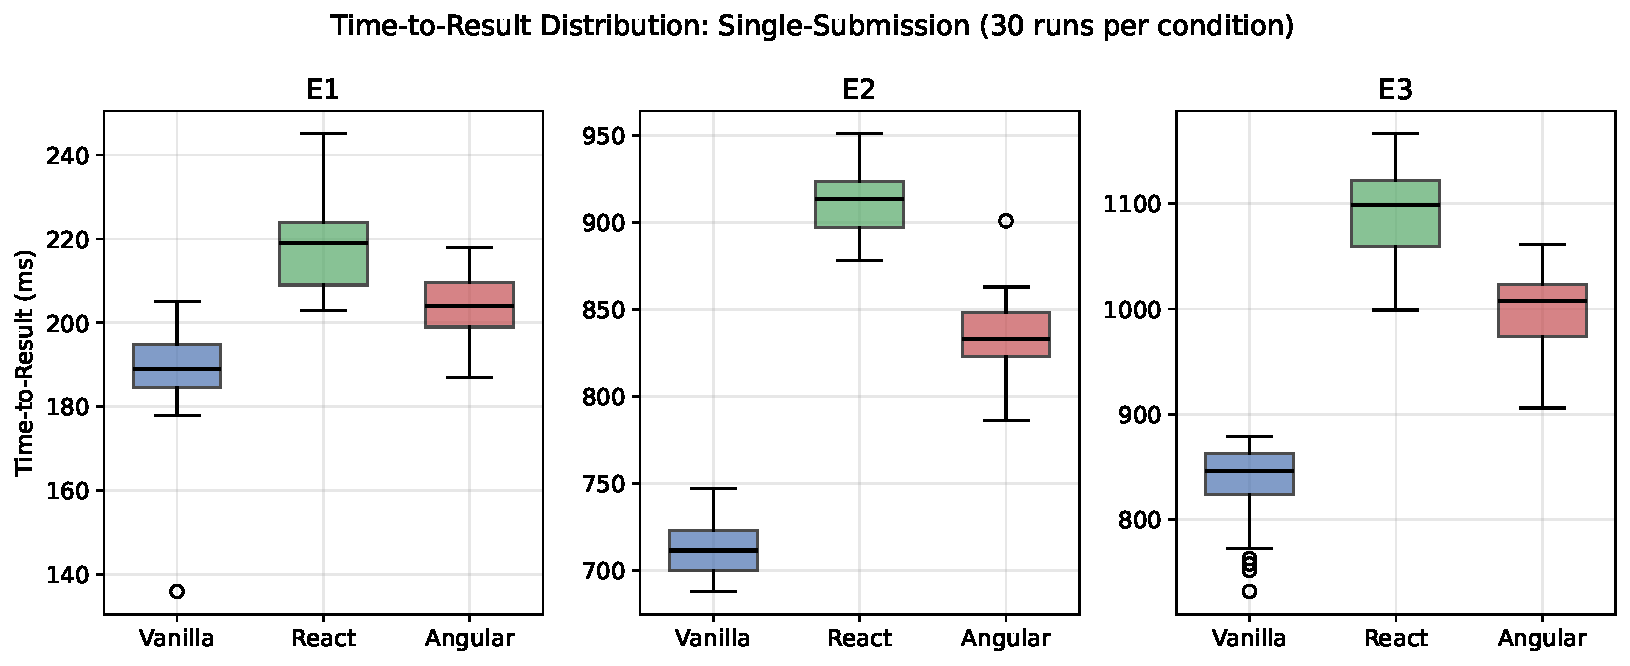
\includegraphics[width=\textwidth]{figures/fig_box_single_submission.pdf}
\caption{Time-to-Result distribution by framework and environment, single-submission scenario (30 runs per condition).}
\label{fig:box-single-submission}
\end{figure}

\vspace{5mm}

Across all three environments, Vanilla JavaScript recorded the lowest median Time-to-Result, followed by Angular, then React. All three IQRs are narrow relative to their medians, therefore indicating low measurement noise within each condition. 

\vspace{5mm}

\subsection{Time-to-Interactive}

Table~\ref{tab:tti-summary} describes the Time-to-Interactive figures. Unlike the above Time-to-Result numbers, TTI values for for React and Angular are noticably closer to eachother than to Vanilla JavaScript's, and all 3 show a substantiallly steeper relative increase from E1 to E3 than Time-to-Result does, this pattern is examined further in Section~\ref{sec:tti-pattern}.

\vspace{5mm} 

\begin{table}[H]
\centering
\caption{Time-to-Interactive (ms), single-submission scenario}
\label{tab:tti-summary}
\begin{tabular}{lccc}
\toprule
Framework & E1 (median) & E2 (median) & E3 (median) \\
\midrule
Vanilla  & 37.5 & 354.0 & 410.0 \\
React    & 47.0 & 445.0 & 500.5 \\
Angular  & 51.5 & 464.5 & 562.0 \\
\bottomrule
\end{tabular}
\end{table}
 
\vspace{5mm}

\begin{figure}[H]
\centering
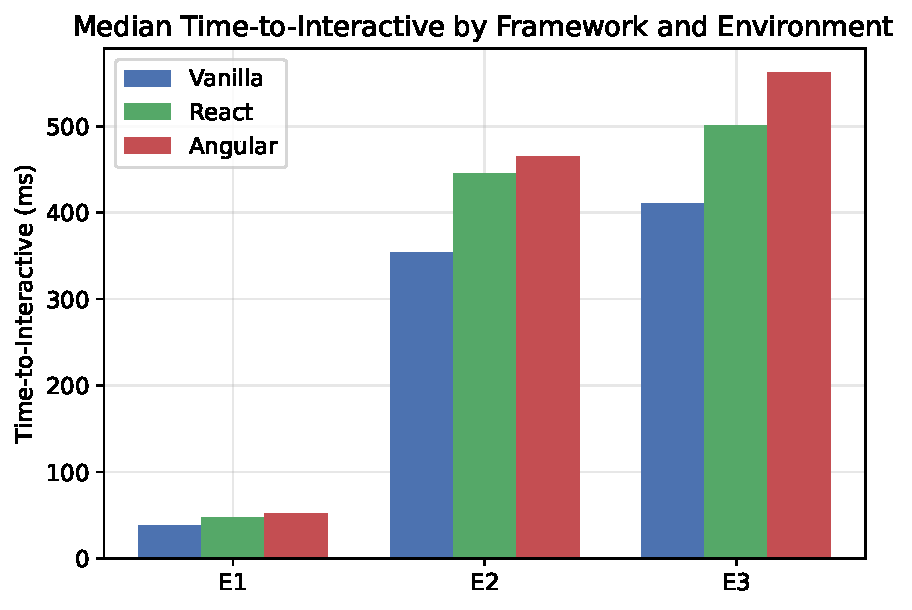
\includegraphics[width=0.8\textwidth]{figures/fig_tti_single_submission.pdf}
\caption{Median Time-to-Interactive by framework and environment, single-submission scenario.}
\label{fig:tti-single-submission}
\end{figure}

\vspace{5mm}

\subsection{Peak Heap Memory}

Table~\ref{tab:heap-summary} showcases peak JavaScript heap memory usage. Angular is consistently shown to have the highest peak heap usage, followed by React, then Vanilla JavaScript, across all three environments. This closely aligns with Angular's more feature-rich run-time, which we discussed previously in Chapter~\ref{ch:background}.

\vspace{5mm}

\begin{table}[H]
\centering
\caption{Peak heap memory (KB), single-submission scenario}
\label{tab:heap-summary}
\begin{tabular}{lccc}
\toprule
Framework & E1 (median) & E2 (median) & E3 (median) \\
\midrule
Vanilla  & 2062.5 & 2497.0 & 2075.0 \\
React    & 2852.0 & 2876.0 & 3286.5 \\
Angular  & 3077.0 & 3061.0 & 3485.0 \\
\bottomrule
\end{tabular}
\end{table}


\vspace{5mm}

\begin{figure}[H]
\centering
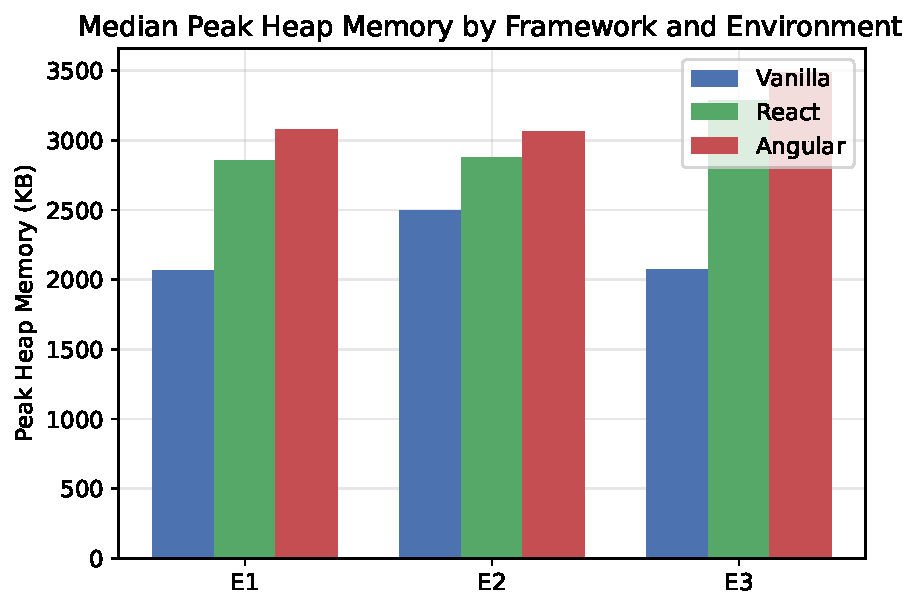
\includegraphics[width=0.8\textwidth]{figures/fig_heap_single_submission.pdf}
\caption{Median peak heap memory by framework and environment, single-submission scenario.}
\label{fig:heap-single-submission}
\end{figure}

\vspace{5mm}

\subsection{Bundle Size}

Unlike the three metrics above, bundle size was measured once per framework from production build output, instead of across repeated runs. This was a deliberate choice as bundle size does not vary between executions. React's production build measured 60.59KB (gzip-compressed), Angular's measured 42.54KB (estimated transfer size). Vanilla JavaScript ships no framework code at all, and its bundle consists only of the application's own
\texttt{script.js}, negligible by comparison.

\subsection{Results Across the Remaining Scenarios}
\label{sec:other-scenarios}

Single-submission was presented above in full detail as the primary, representative scenario. The remaining three scenarios, cold-load, stress-test, and error-handling follow the same overall framework ordering, with Vanilla JavaScript consistently outperforming Angular and React, with the two frameworks carrying measurable overhead. However, the remaining scenarios differ in absolute magnitude and sometimes in relative ordering between React and Angular. Tables~\ref{tab:coldload},
\ref{tab:stresstest}, and~\ref{tab:errorhandling} report the median of each metric for these three scenarios, interquartile ranges are omitted here for formatting reasons, but follow the same narrow spread pattern observed in Single-submission data, and are available in full in the accompanying code submission. 

\begin{table}[H]
\centering
\caption{Cold-load scenario: median TTR (ms), TTI (ms), peak heap (KB)}
\label{tab:coldload}
\begin{tabular}{llccc}
\toprule
Environment & Framework & TTR & TTI & Peak Heap \\
\midrule
\multirow{3}{*}{E1} & Vanilla & 36.0  & 34.0  & 1085.0 \\
                     & React   & 60.0  & 46.0  & 1627.0 \\
                     & Angular & 54.0  & 52.0  & 1987.0 \\
\midrule
\multirow{3}{*}{E2} & Vanilla & 359.0 & 355.5 & 1085.0 \\
                     & React   & 523.5 & 442.5 & 1627.0 \\
                     & Angular & 474.0 & 470.0 & 1987.0 \\
\midrule
\multirow{3}{*}{E3} & Vanilla & 424.0 & 414.0 & 1085.0 \\
                     & React   & 655.0 & 506.0 & 1627.0 \\
                     & Angular & 576.0 & 569.5 & 1987.0 \\
\bottomrule
\end{tabular}
\end{table}

\vspace{5mm}

\begin{figure}[H]
\centering
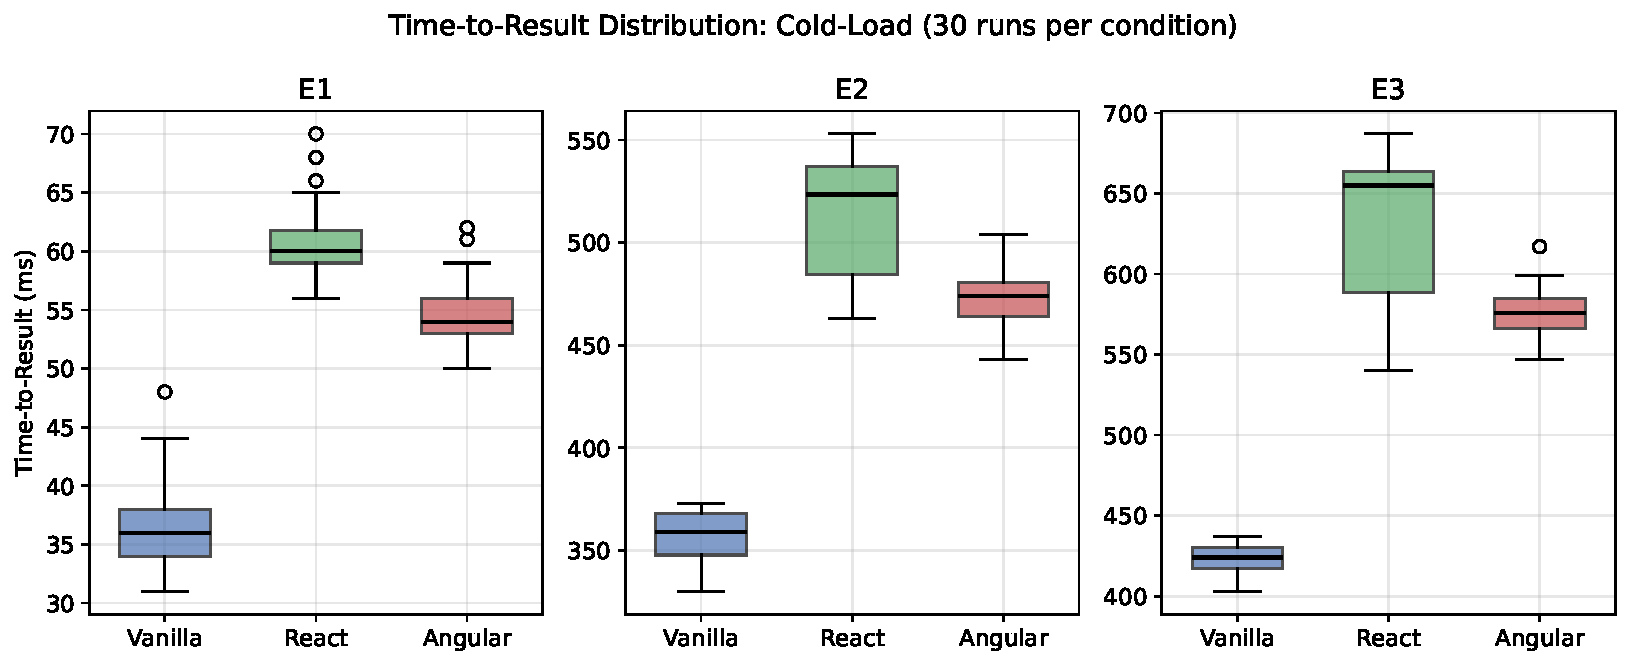
\includegraphics[width=\textwidth]{figures/fig_box_coldload.pdf}
\caption{Time-to-Result distribution by framework and environment, cold-load scenario (30 runs per condition).}
\label{fig:box-coldload}
\end{figure}

\vspace{5mm}

Cold-load's peak heap values are the most stable in the entire dataset, each implementation recorded a consistent value across all three environments, Vanilla JavaScript with 1085KB, 1627KB for React, and 1987KB for Angular. This stability was expected, as the scenario involves no user interaction, meaning memory usage reflects only each framework's static runtime footprint, with no interaction-dependent allocation to introduce variation. This perfect within-group consistency is also the source of the Cohen's d zero-variance edge case described in Chapter~\ref{ch:implementation}.

\vspace{5mm}

\begin{table}[H]
\centering
\caption{Stress-test scenario: median TTR (ms), TTI (ms), peak heap (KB)}
\label{tab:stresstest}
\begin{tabular}{llccc}
\toprule
Environment & Framework & TTR & TTI & Peak Heap \\
\midrule
\multirow{3}{*}{E1} & Vanilla & 566.5  & 36.5  & 2392.0 \\
                     & React   & 604.5  & 46.0  & 3224.0 \\
                     & Angular & 506.0  & 51.5  & 3353.0 \\
\midrule
\multirow{3}{*}{E2} & Vanilla & 1364.5 & 355.5 & 2465.5 \\
                     & React   & 1544.5 & 445.5 & 3186.5 \\
                     & Angular & 1289.0 & 468.0 & 3616.5 \\
\midrule
\multirow{3}{*}{E3} & Vanilla & 1507.5 & 408.0 & 2850.0 \\
                     & React   & 1799.0 & 505.0 & 3308.5 \\
                     & Angular & 1691.5 & 568.0 & 3516.0 \\
\bottomrule
\end{tabular}
\end{table} 

\vspace{5mm}

\begin{figure}[H]
\centering
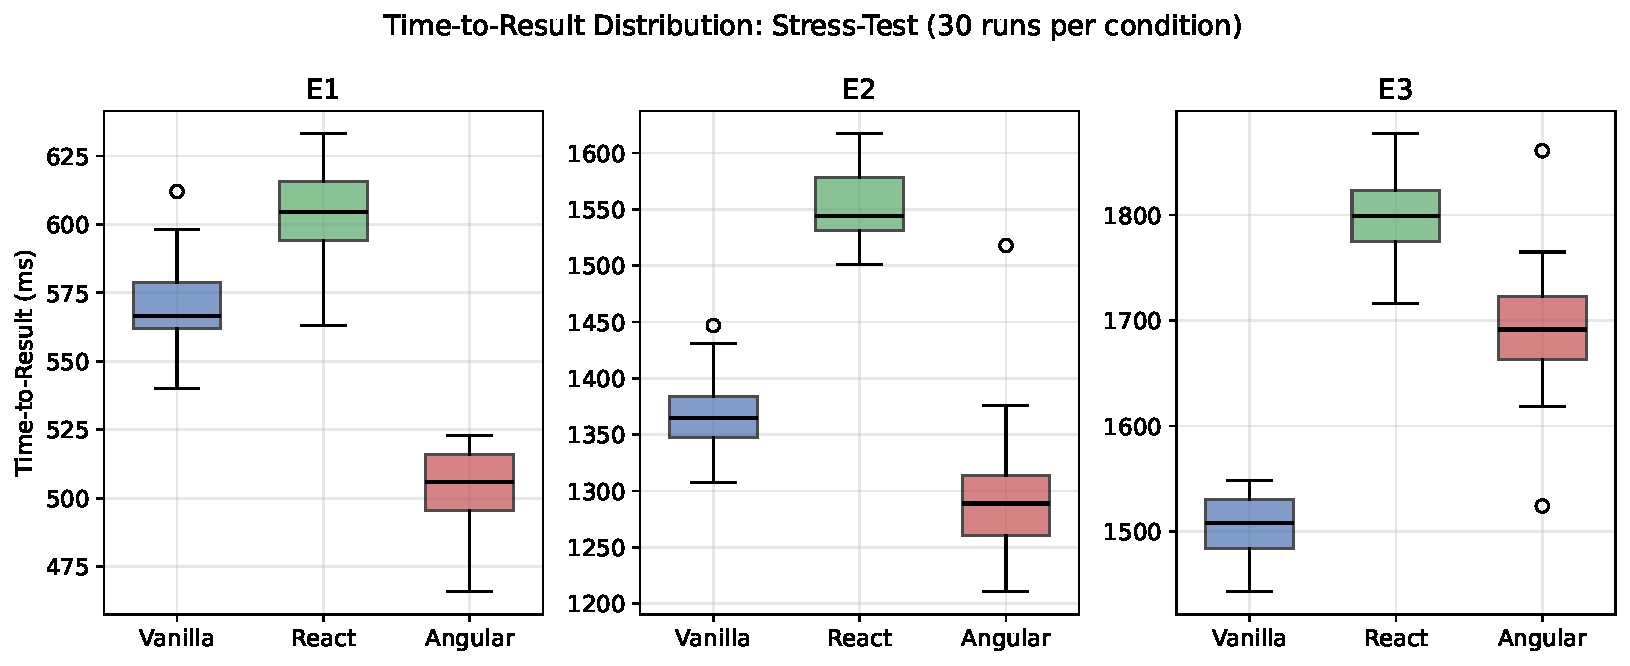
\includegraphics[width=\textwidth]{figures/fig_box_stresstest.pdf}
\caption{Time-to-Result distribution by framework and environment, stress-test scenario (30 runs per condition). Note Angular's lower median at E1 and E2, the exception to the general framework ordering discussed in Section~\ref{sec:framework-ordering}.}
\label{fig:box-stresstest}
\end{figure}


\vspace{5mm}

The stress-test scenario represents an exception to the framework ordering observed across all other scenarios. At both E1 and E2, Angular achieves the lowest median Time-to-Result, outperforming Vanilla. However, this finding does not extend to E3, where the familiar ordering observed everywhere else continues. The implications of this anomoly are discussed in Section~\ref{sec:framework-ordering}.


\begin{table}[H]
\centering
\caption{Error-handling scenario: median TTR (ms), TTI (ms), peak heap (KB)}
\label{tab:errorhandling}
\begin{tabular}{llccc}
\toprule
Environment & Framework & TTR & TTI & Peak Heap \\
\midrule
\multirow{3}{*}{E1} & Vanilla & 126.5 & 36.5  & 2009.0 \\
                     & React   & 149.0 & 47.0  & 2591.0 \\
                     & Angular & 146.0 & 52.0  & 2884.0 \\
\midrule
\multirow{3}{*}{E2} & Vanilla & 514.5 & 361.0 & 2542.0 \\
                     & React   & 716.0 & 455.0 & 3347.5 \\
                     & Angular & 640.0 & 474.5 & 3099.5 \\
\midrule
\multirow{3}{*}{E3} & Vanilla & 657.5 & 418.0 & 2120.0 \\
                     & React   & 937.5 & 517.5 & 3346.0 \\
                     & Angular & 830.5 & 580.0 & 3519.0 \\
\bottomrule
\end{tabular}
\end{table}

\vspace{5mm}

\begin{figure}[H]
\centering
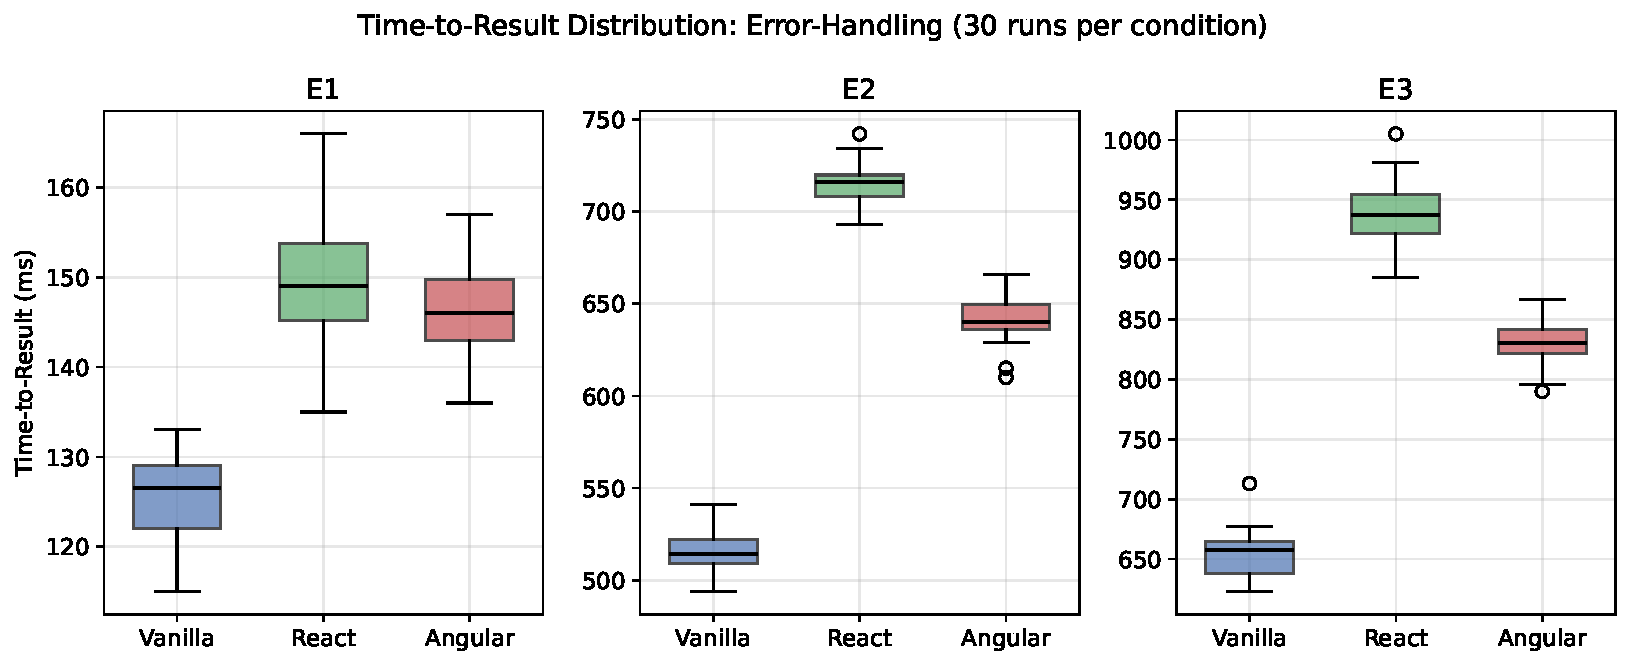
\includegraphics[width=\textwidth]{figures/fig_box_errorhandling.pdf}
\caption{Time-to-Result distribution by framework and environment, error-handling scenario (30 runs per condition).}
\label{fig:box-errorhandling}
\end{figure}

\vspace{5mm}

The error-handling scenario records the fastest absolute Time-to-Result of any non-cold-load scenario. This is unsurprising, as a failed request is resolved immediately upon network failure, bypassing the model inference stage entirely, unlike a successful submission, which must wait for the full classification pipeline to complete.

\section{Statistical Testing}

\subsection{Kruskal-Wallis Results}

\vspace{5mm}

All 36 scenario/environment/metric combinations returned a statistically significant result under the Kruskal-Wallis test after the Bonferroni correction, with p-values uniformly below the adjusted threshold of $\alpha = 0.00139$ in every case. This indicates that, across every scenario, environment, and metric tested, the three frameworks' performance distributions differ significantly from one another. Given that every comparison reached significance, statistical significance alone does not distinguish between the 36 results in terms of practical importance, this is the role of the statistical measure Cohen's d, which is discussed in the next section.   

\subsection{Pairwise Comparisons and Effect Sizes}

\vspace{5mm}

Pairwise Mann-Whitney U tests were run for every significant Kruskal-Wallis result, and Cohen's d was calculated for each pairwise comparison. The overwhelming majority of pairwise comparisons produced large effect sizes, with Cohen's d values surpassing the conventional $|d| > 0.8$ criterion for a large effect. This finding is consistent with the tight IQRs observed in Chapter~\ref{ch:results}, with low within-group variance, even modest absolute differences between frameworks translate into large standardised effect sizes. 

\vspace{5mm}

A small number of comparisons involved metrics with zero or near-zero variance within one or both groups, most notably peak heap memory during the cold-load scenario, where both Vanilla JavaScript's heap usage at 1085KB and Angular's heap usage at 1987KB were identical across all 30 runs at every environment. React's heap usage was almost as stable, ranging between 1626--1627KB in nearly all
runs, with one isolated 2251KB outlier. For these cases, Cohen's d is mathematically undefined or numerically unstable, as described in Chapter~\ref{ch:implementation}, and the raw mean difference is reported in its place. For example, Vanilla JavaScript and Angular's cold-load peak heap memory differed by a consistent 902KB across all 30 runs at every environment, with zero overlap between the two distributions.
This difference is just as reliable as any other result in the dataset, despite not admitting a conventional Cohen's d value.

\section{Degradation Gradient}

Table~\ref{tab:degradation} shows the ratio of each framework's E3 median
to its E1 median, for Time-to-Result, across all four scenarios.

\begin{table}[H]
\centering
\caption{Degradation ratio (E3 median / E1 median), Time-to-Result}
\label{tab:degradation}
\begin{tabular}{lccc}
\toprule
Scenario & Vanilla & React & Angular \\
\midrule
Cold Load           & 11.78x & 10.92x & 10.67x \\
Single Submission    & 4.48x  & 5.02x  & 4.94x \\
Stress Test          & 2.66x  & 2.98x  & 3.34x \\
Error Handling       & 5.20x  & 6.29x  & 5.69x \\
\bottomrule
\end{tabular}
\end{table}

\vspace{5mm}

\begin{figure}[H]
\centering
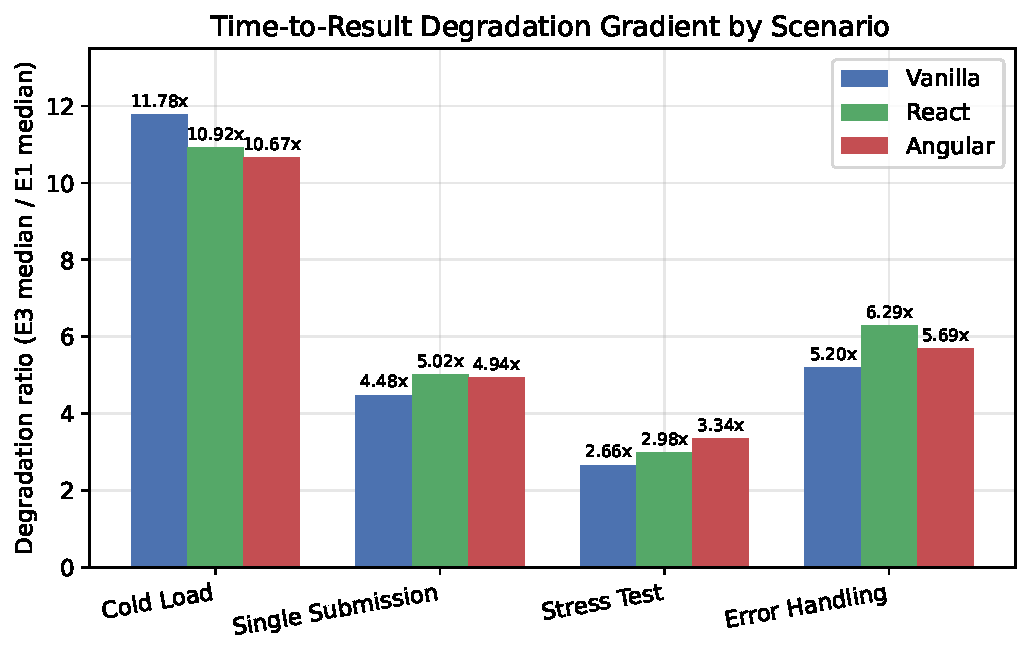
\includegraphics[width=0.85\textwidth]{figures/fig_degradation_gradient.pdf}
\caption{Time-to-Result degradation ratio (E3 median / E1 median) by scenario and framework.}
\label{fig:degradation-gradient}
\end{figure}

\vspace{5mm}

There are two patterns apparent within this table. First, within each scenario, the three frameworks degradation ratios are relatively close to one another, for
example, 4.48x--5.02x for single-submission. This indicates that environment, not framework choice, is the dominant factor in driving total performance change from E1 to E3. Second, the ranking of frameworks by degradation ratio is not perfectly consistent across scenarios,
React degrades the most in single-submission and error-handling, but Angular degrades the most in stress-test, suggesting that which framework is most affected by constrained conditions may depend on the specific  interaction pattern being tested, not on a single fixed ordering


\section{Discussion}

\subsection{Answering the Research Question}

\vspace{5mm}

The results presented in this chapter provide the basis for answering the three research questions initially posed in Chapter~\ref{ch:introduction}. RQ1 inquired whether the three frameworks exhibit differential load-time performance and whether any such differences are modulated by device specifications. The findings indicate significant differences across all environments tested, with Vanilla JavaScript consistently achieving the lowest latency, while React and Angular each introduce a measurable and statistically significant overhead. The magnitude of this overhead varies with the environment, although the relative ordering of the frameworks remains broadly invariant. 

\vspace{5mm}

RQ2 turned specifically to memory consumption and Time-to-Result. Peak heap memory differences between frameworks are present but proportionally minor compared to the Time-to-Result differentials, and remain comparatively stable across environments, increasing by a factor of only 1.0x to 1.3x from E1 to E3. By contrast, Time-to-Result differences are pronounced and widen substantially under constrained conditions. 

\vspace{5mm}

RQ3 questioned whether a threshold exists below which framework overhead becomes prohibitive for classroom use. This question is considered, with appropriate qualifications, in Section~\ref{sec:limitations}.

\subsection{The TTI Degradation Pattern}
\label{sec:tti-pattern}

\vspace{5mm}

Comparing TTI's degradation ratio to that of Time-to-Result revealed a notable distinction. TTI degrades by a remarkably consistent factor of 10.6x to 12.2x from E1 to E3, regardless of framework or scenario. Time-to-Result's degradation ratio, on the other hand, varies a lot more, ranging from 2.66x to 11.78x depending on both framework and scenario.

\vspace{5mm}

This contrast suggests that the TTI proxy used in this study is capturing something close to a pure CPU-throttle effect. Defined as the time until the page's load event fires plus one animation frame, TTI is dominated by JavaScript parse and execution time. However, Time-to-Result spans the full round trip to the backend and back, thereby capturing network-dependent and framework dependent variation that TTI does not. 

\vspace{5mm}

This observation suggests that the TTI proxy, on its own, is not well suited to isolating framework-specific overhead, and that Time-to-Result remains the more informative metric for directly answering RQ1 and RQ2.

\vspace{5mm}

\begin{figure}[H]
\centering
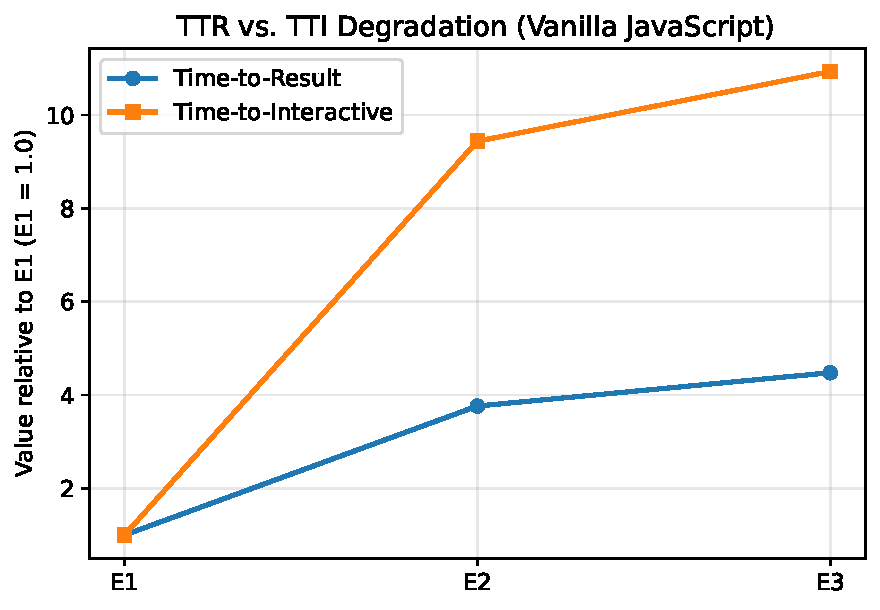
\includegraphics[width=0.8\textwidth]{figures/fig_ttr_vs_tti_pattern.pdf}
\caption{Time-to-Result and Time-to-Interactive degradation, normalised to E1 (Vanilla JavaScript). TTI degrades almost independently of environment scaling in a manner distinct from TTR.}
\label{fig:ttr-vs-tti-pattern}
\end{figure}

\vspace{5mm}

\subsection{Framework Ordering and Consistency}
\label{sec:framework-ordering}

\vspace{5mm}

Across most scenarios, environments, and metrics measured, a consistent ordering holds. Vanilla JavaScript has proved itself to perform best, with both React and Angular carrying a measurable, statistically significant overhead. This ordering appears in the descriptive statistics presented in earlier sections in this chapter, and is confirmed as statistically significant in the corresponding Kruskal-Wallis tests, and persists across three of the four scenarios tested. 

\vspace{5mm}

The stress-test scenario constitutes a genuine exception. At E1 and E2, Angular records the lowest median Time-to-Result of the three frameworks, surpassing Vanilla JavaScript, as shown in Table~\ref{tab:stresstest}. A genuine explanation for this is that Angular Signal's change notification may handle the five closely spaced state updates in this scenario more efficiently than Vanilla JavaScript's manually-triggered DOM updates, which re-run their full rendering logic on every submission regardless of how much has actually changed. This remains a plausible explanation rather than a confirmed mechanism, as this study did not directly instrument each framework's internal update behaviour. It is noted as an unresolved point of interest rather than a contradiction to be explained. 

\vspace{5mm}

The general Vanilla-fastest ordering established above has proved itself to be consistent, is confirmed to be statistically significant in every relevant Kruskal-Wallis test, and persists across three of the four scenarios tested, suggesting it reflects a genuine, stable property of the frameworks' runtime behaviour under the conditions tested, rather than an artefact of any single measurement

\subsection{Limitations}
\label{sec:limitations}

\vspace{5mm}

Several limitations of this study should be acknowledged when interpreting its results. While the design choices were intended to provide a controlled comparisons between the 3 implementations, certain factors may have influenced the measured performance outcomes. These limitations should therefore be considered when assessing the extent to which the above findings can generalise to other use cases. 

\vspace{5mm}

The TTI metric is a proxy, not a full Lighthouse measurement. As described in Chapter~\ref{ch:implementation}, Time-to-Interactive was approximated as the point at which the page's load event fires plus one animation frame, rather than using Lighthouse's full TTI algorithm, which additionally requires a window of network and main-thread inactivity. This proxy was chosen because running full Lighthouse audits for all 1,080 individual runs would have been impractically slow. Consequently, the absolute TTI values reported here should not be directly compared against published Lighthouse scores for other applications. Instead, they are valid for comparing the three frameworks against each other under identical conditions, because the same proxy was applied consistently across all measurements. 

\vspace{5mm}

The production-build discovery narrows what this study can claim. As described in Chapter~\ref{ch:implementation}, only the corrected, production-build measurements are reported in this chapter. The study makes no claim about relative framework performance under development-server conditions, which represent a different, and less representative of real deployment, comparison. 

\vspace{5mm}

RQ3's threshold question is only partially answerable with three discrete environments. E1,E2, and E3 represent three specific points along a hardware and network constraint spectrum, not a continuous sweep. The degradation gradeitn analysis in this chapter is able to characterise how the performance gap between frameworks changes across these three points, but is not able to pinpoint an exact constraint level at which a framework becomes "unsuitable", since no data exists between or beyond these three sampled conditions. 

\vspace{5mm}


% ============================================================
\chapter{Project Management}
\label{ch:project-management}

\section{Timeline and Progress}

\vspace{5mm}

The dissertation project was structured around a 24-week timeline that was briefly described in Chapter~\ref{ch:approach}, divided into six phases, literature review and project scaffolding (weeks 1-4), Vanilla JavaScript and React implementation (weeks 5-8), Angular implementation and full validation (weeks 9-12),  benchmarking harness construction and data collection (weeks 13-16), statistical analysis (weeks 17-20), and dissertation
write-up (weeks 21-24).

\vspace{5mm}

The project closely followed the proposed 24-week timeline. By the interim report submission at the boundary of weeks 9-12, all three front-end implementations and the backend had been built and validated, matching the plan exactly. The sole deviation from the original plan was the mid-phase pivot from a hosted Hugging Face Inference API to a self-hosted backend, described in Chapter~\ref{ch:implementation}, this change was accommodated within the same phase and did not impact the overall schedule. The benchmarking harness was built and all 1,080 individual runs were collected within weeks 13-16 as planned, and the full statistical analysis, including the discovery and resolution of the cold-load heap measurement gap and the Cohen's d zero variance edge case, was completed within weeks 17-20.

\vspace{5mm}

\section{Version Control and Code Management}

\vspace{5mm}

All source code is version controlled using Git and hosted on GitHub\footnote{\url{https://github.com/kav51/Masters-Diss-App}}. A \texttt{.gitignore} configuration excludes dependency directories (\texttt{node\_modules}, Python virtual environments) from version control, ensuring the repository remains focused on authored source code rather than reinstallable third-party packages.

\vspace{5mm}

Commits were made upon the completion of each major component, including the backend, each frontend implementation, the benchmarking harness, and the statistical analysis pipeline, once local testing had been performed, rather than through frequent incremental commits during development.

% ============================================================
\chapter{Appraisal and Reflection}
\label{ch:appraisal}

\section{Goals Achieved}    

All three questions introduced in Chapter~\ref{ch:introduction} were answered empirically, using a statistically validated dataset of 1,080 benchmark runs across the three implementations, three environments, and four scenarios. All four of the contributions promised in Chapter~\ref{ch:introduction} were delivered. This includes the three functionally indentical frontend implementations, a reusable automated benchmarking harness, the full dataset and statistical analysis, and an answer to each research question.   

\vspace{5mm}

RQ3, which addressed whether a specific device constraint threshold exists below which any framework becomes unsuitable, was answered only partially, as discussed in Chapter~\ref{ch:results}, Section~\ref{sec:limitations}. The three discrete environments tested allow the degradation gradient to be characterised, but do not permit a precise threshold to be pinpointed. This is a scope limitation, rather than an unmet goal, because a continuous sweep of hardware conditions was never part of the original experiment design. 

\section{Lessons Learned}

Throughout the dissertation, I encountered several unexpected problems that, while initially disruptive, provided valuable learning experiences. Both the HuggingFace API unavailability and the Angular's zoneless change-detection issue required diagnosing a problem methodically, for example narrowing down where in the pipeline a fault occurred, this discipline carried forward directly into more subtle bugs that were found later in the cold-load heap measurement gap and the Cohen's d zero-variance edge case. Both of the cases were only caught through careful inspection of results that seemed deceptively plausible but on closer examination were not correct.


\section{What Would Be Done Differently}

Several aspects of this dissertation project could have been improved in hindsight. Firstly, adopting a more detailed commit history would improve traceability and would simplify the development process narrative. Secondly, a wider range of test text would capture how framework performance behaves under more diverse, realistic usage. Third, sampling additional thorttling levels beyond the three discrete environments would enablle a more precise characterisation of the degradation gradient and a more definitive answer to RQ3. Finally, a more detailed analysis of framework internals would allow for plausible explanations to be confirmed or rejected with greater confidence.
In retrospect, regular supervisor meetings would have benefited immensely. Earlier feedback would have proved useful in terms of experiment design.
% ============================================================
\chapter{Ethics}
\label{ch:ethics}

This project does not involve human participants, personal data, or any other form of sensitive data. All benchmarking was conducted using an automated browser tooling (Playwright), submitting fixed, pre-selected text samples to a locally run classifier. There was at no point any real student's writing, or any other personal data collected, stored, and processed.

\vspace{5mm}

The pretrained CEFR classification model used in this project was used strictly as a fixed component. There was no model training, fine-tuning or any use of proprietary/restricted training data undertaken as part of this project. No ethical approval was required for this dissertation project under the University's ethical consent guidelines. This position was not revisited during the dissertation, as  no aspect of the work introduced human participants or personal data. 


% ============================================================
\chapter{AI Usage}
\label{ch:ai-usage}

Artificial Intelligence was used minimally and critically throughout this project. AI assistence was used to assist in diagnosing the four problems described in Chapter~\ref{ch:implementation}, by providing suggestions that helped to narrow down potential causes. Each diagnosis was independently verified and tested, in order to ensure that the underlying cause of each issue was understood. 
% ============================================================
\chapter{Conclusion}
\label{ch:conclusion}

\section{Summary of Findings}

The aim of this dissertation was to answer whether the choice of frontend JavaScript framework measurably affects the performance of a realistic, NLP-driven educational web application under simulated classroom computing constraints. Three functionally identical implementations, Vanilla JavaScript, React, and Angular, were built around an identical backend which served a pretrained CEFR classification model, and benchmarked across three simulated hardware/network environments, four usage scenarios, and four performmance metrics, totalling 1,080 individual runs. 

\vspace{5mm}

The results clearly show that frontend framework choice does produce a measurable, statistically significant difference in application responsiveness, consistently across every scenario, environment, and metric tested. Vanilla JavaScript performed best in the majority of conditions, with React and Angular each carrying measurable overhead. Angular consistently outperformed React on Time-to-Result, despite also recording the highest peak heap memory usage of the three implementations. The magnitude of the performance gap between the three was quite small relative to the overall effect of the environmental constraint, moving from E1 to E3 degraded performance far more than switching frameworks did. However, there was one exception, uncovered by the stress-test scenario, where Angular outperformed Vanilla JavaScript in the least constrained environments. A further finding states that Time-to-Interactive degrades under throttling and does so almost entirely independently of framework choice, whereas Time-to-Result's degradation varies substantially with both framework and scenario. This suggests that Time-to-Result, not Time-to-Interactive, is the more informative metric for studies of this kind. Taken together, these findings confirm that framework choice matters, but practical significance of these respective advantages are heavily moderated by the device environment. For developers that are building educational tools for low-end classroom devices, the findings suggest that framework selection should be informed by the specific usage patterns and constraints of the target context, instead of by developer familiarity or ecosystem popularity.

\section{Future Work}

In concluding this dissertation, I can observe several directions that follow naturally from the limitations discussed in Chapter~\ref{ch:results}, Section~\ref{sec:limitations}. Firstly, a continuous sweep of hardware/network constraint levels, rather than three discrete environments, would allow RQ3's threshold question to be answered more precisely. Testing with a range of submission text lengths and content types, rather than a single fixed sentence would establish whether the findings reported here generalise beyond the specific workload tested. Finally, replacing the Time-to-Interactive proxy used in this study with full Lighthouse audits, for at least a representative subset of runs, would allow the TTI degradation pattern identified in Chapter~\ref{ch:results} to be validated against an industry-standard measurement.

% ============================================================
\printbibliography

% ============================================================
\appendix
\chapter{Additional Material}
% TODO: e.g. extra data tables, code excerpts too long for the main text

\end{document}